\documentclass[twoside]{book}

% Packages required by doxygen
\usepackage{fixltx2e}
\usepackage{calc}
\usepackage{doxygen}
\usepackage[export]{adjustbox} % also loads graphicx
\usepackage{graphicx}
\usepackage[utf8]{inputenc}
\usepackage{makeidx}
\usepackage{multicol}
\usepackage{multirow}
\PassOptionsToPackage{warn}{textcomp}
\usepackage{textcomp}
\usepackage[nointegrals]{wasysym}
\usepackage[table]{xcolor}

% Font selection
\usepackage[T1]{fontenc}
\usepackage[scaled=.90]{helvet}
\usepackage{courier}
\usepackage{amssymb}
\usepackage{sectsty}
\renewcommand{\familydefault}{\sfdefault}
\allsectionsfont{%
  \fontseries{bc}\selectfont%
  \color{darkgray}%
}
\renewcommand{\DoxyLabelFont}{%
  \fontseries{bc}\selectfont%
  \color{darkgray}%
}
\newcommand{\+}{\discretionary{\mbox{\scriptsize$\hookleftarrow$}}{}{}}

% Page & text layout
\usepackage{geometry}
\geometry{%
  a4paper,%
  top=2.5cm,%
  bottom=2.5cm,%
  left=2.5cm,%
  right=2.5cm%
}
\tolerance=750
\hfuzz=15pt
\hbadness=750
\setlength{\emergencystretch}{15pt}
\setlength{\parindent}{0cm}
\setlength{\parskip}{3ex plus 2ex minus 2ex}
\makeatletter
\renewcommand{\paragraph}{%
  \@startsection{paragraph}{4}{0ex}{-1.0ex}{1.0ex}{%
    \normalfont\normalsize\bfseries\SS@parafont%
  }%
}
\renewcommand{\subparagraph}{%
  \@startsection{subparagraph}{5}{0ex}{-1.0ex}{1.0ex}{%
    \normalfont\normalsize\bfseries\SS@subparafont%
  }%
}
\makeatother

% Headers & footers
\usepackage{fancyhdr}
\pagestyle{fancyplain}
\fancyhead[LE]{\fancyplain{}{\bfseries\thepage}}
\fancyhead[CE]{\fancyplain{}{}}
\fancyhead[RE]{\fancyplain{}{\bfseries\leftmark}}
\fancyhead[LO]{\fancyplain{}{\bfseries\rightmark}}
\fancyhead[CO]{\fancyplain{}{}}
\fancyhead[RO]{\fancyplain{}{\bfseries\thepage}}
\fancyfoot[LE]{\fancyplain{}{}}
\fancyfoot[CE]{\fancyplain{}{}}
\fancyfoot[RE]{\fancyplain{}{\bfseries\scriptsize Generated by Doxygen }}
\fancyfoot[LO]{\fancyplain{}{\bfseries\scriptsize Generated by Doxygen }}
\fancyfoot[CO]{\fancyplain{}{}}
\fancyfoot[RO]{\fancyplain{}{}}
\renewcommand{\footrulewidth}{0.4pt}
\renewcommand{\chaptermark}[1]{%
  \markboth{#1}{}%
}
\renewcommand{\sectionmark}[1]{%
  \markright{\thesection\ #1}%
}

% Indices & bibliography
\usepackage{natbib}
\usepackage[titles]{tocloft}
\setcounter{tocdepth}{3}
\setcounter{secnumdepth}{5}
\makeindex

% Hyperlinks (required, but should be loaded last)
\usepackage{ifpdf}
\ifpdf
  \usepackage[pdftex,pagebackref=true]{hyperref}
\else
  \usepackage[ps2pdf,pagebackref=true]{hyperref}
\fi
\hypersetup{%
  colorlinks=true,%
  linkcolor=blue,%
  citecolor=blue,%
  unicode%
}

% Custom commands
\newcommand{\clearemptydoublepage}{%
  \newpage{\pagestyle{empty}\cleardoublepage}%
}

\usepackage{caption}
\captionsetup{labelsep=space,justification=centering,font={bf},singlelinecheck=off,skip=4pt,position=top}

%===== C O N T E N T S =====

\begin{document}

% Titlepage & ToC
\hypersetup{pageanchor=false,
             bookmarksnumbered=true,
             pdfencoding=unicode
            }
\pagenumbering{alph}
\begin{titlepage}
\vspace*{7cm}
\begin{center}%
{\Large My Project }\\
\vspace*{1cm}
{\large Generated by Doxygen 1.8.13}\\
\end{center}
\end{titlepage}
\clearemptydoublepage
\pagenumbering{roman}
\tableofcontents
\clearemptydoublepage
\pagenumbering{arabic}
\hypersetup{pageanchor=true}

%--- Begin generated contents ---
\chapter{Class Index}
\doxysection{Class List}
Here are the classes, structs, unions and interfaces with brief descriptions\+:\begin{DoxyCompactList}
\item\contentsline{section}{\mbox{\hyperlink{structCOORDENADA}{C\+O\+O\+R\+D\+E\+N\+A\+DA}} \\*Tipo de dados para as coordenadas }{\pageref{structCOORDENADA}}{}
\item\contentsline{section}{\mbox{\hyperlink{structESTADO}{E\+S\+T\+A\+DO}} \\*Tipo de dados para o estado }{\pageref{structESTADO}}{}
\item\contentsline{section}{\mbox{\hyperlink{structJOGADA}{J\+O\+G\+A\+DA}} \\*Tipo de dados para a jogada }{\pageref{structJOGADA}}{}
\end{DoxyCompactList}

\chapter{File Index}
\doxysection{File List}
Here is a list of all documented files with brief descriptions\+:\begin{DoxyCompactList}
\item\contentsline{section}{{\bfseries Camada\+\_\+de\+\_\+\+Dados.\+h} }{\pageref{Camada__de__Dados_8h}}{}
\item\contentsline{section}{{\bfseries dados.\+h} }{\pageref{dados_8h}}{}
\item\contentsline{section}{\mbox{\hyperlink{Interface_8h}{Interface.\+h}} }{\pageref{Interface_8h}}{}
\item\contentsline{section}{\mbox{\hyperlink{Logica__do__programa_8h}{Logica\+\_\+do\+\_\+programa.\+h}} }{\pageref{Logica__do__programa_8h}}{}
\end{DoxyCompactList}

\chapter{Class Documentation}
\hypertarget{structCOORDENADA}{}\section{C\+O\+O\+R\+D\+E\+N\+A\+DA Struct Reference}
\label{structCOORDENADA}\index{C\+O\+O\+R\+D\+E\+N\+A\+DA@{C\+O\+O\+R\+D\+E\+N\+A\+DA}}


Tipo de dados para as coordenadas.  




{\ttfamily \#include $<$dados.\+h$>$}

\subsection*{Public Attributes}
\begin{DoxyCompactItemize}
\item 
\mbox{\Hypertarget{structCOORDENADA_adfbc8d4856ce807139fdf62e00aed29a}\label{structCOORDENADA_adfbc8d4856ce807139fdf62e00aed29a}} 
int {\bfseries coluna}
\item 
\mbox{\Hypertarget{structCOORDENADA_aefe14bcc5a066ac3b21500cc3d28c06f}\label{structCOORDENADA_aefe14bcc5a066ac3b21500cc3d28c06f}} 
int {\bfseries linha}
\end{DoxyCompactItemize}


\subsection{Detailed Description}
Tipo de dados para as coordenadas. 

The documentation for this struct was generated from the following file\+:\begin{DoxyCompactItemize}
\item 
dados.\+h\end{DoxyCompactItemize}

\hypertarget{structESTADO}{}\doxysection{E\+S\+T\+A\+DO Struct Reference}
\label{structESTADO}\index{ESTADO@{ESTADO}}


Tipo de dados para o estado.  




{\ttfamily \#include $<$dados.\+h$>$}



Collaboration diagram for E\+S\+T\+A\+DO\+:

\hypertarget{structJOGADA}{}\section{J\+O\+G\+A\+DA Struct Reference}
\label{structJOGADA}\index{J\+O\+G\+A\+DA@{J\+O\+G\+A\+DA}}


Tipo de dados para a jogada.  




{\ttfamily \#include $<$dados.\+h$>$}



Collaboration diagram for J\+O\+G\+A\+DA\+:
\nopagebreak
\begin{figure}[H]
\begin{center}
\leavevmode
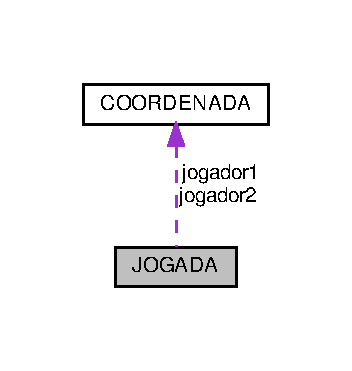
\includegraphics[width=169pt]{structJOGADA__coll__graph}
\end{center}
\end{figure}
\subsection*{Public Attributes}
\begin{DoxyCompactItemize}
\item 
\mbox{\Hypertarget{structJOGADA_a93d9306cb0c49b66b7d9a615bffe0149}\label{structJOGADA_a93d9306cb0c49b66b7d9a615bffe0149}} 
\hyperlink{structCOORDENADA}{C\+O\+O\+R\+D\+E\+N\+A\+DA} {\bfseries jogador1}
\item 
\mbox{\Hypertarget{structJOGADA_ab46b16dfbdc7f2af9430c8dcdac0914b}\label{structJOGADA_ab46b16dfbdc7f2af9430c8dcdac0914b}} 
\hyperlink{structCOORDENADA}{C\+O\+O\+R\+D\+E\+N\+A\+DA} {\bfseries jogador2}
\end{DoxyCompactItemize}


\subsection{Detailed Description}
Tipo de dados para a jogada. 

The documentation for this struct was generated from the following file\+:\begin{DoxyCompactItemize}
\item 
dados.\+h\end{DoxyCompactItemize}

\hypertarget{structlista}{}\section{lista Struct Reference}
\label{structlista}\index{lista@{lista}}


Collaboration diagram for lista\+:
\nopagebreak
\begin{figure}[H]
\begin{center}
\leavevmode
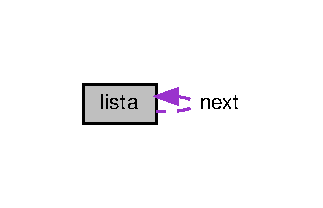
\includegraphics[width=155pt]{structlista__coll__graph}
\end{center}
\end{figure}
\subsection*{Public Attributes}
\begin{DoxyCompactItemize}
\item 
\mbox{\Hypertarget{structlista_a1851230b0237deef0519ee33de9f2dd0}\label{structlista_a1851230b0237deef0519ee33de9f2dd0}} 
void $\ast$ {\bfseries valor}
\item 
\mbox{\Hypertarget{structlista_a03e6d0ed2ba4b439580ef0dcdb0b20c4}\label{structlista_a03e6d0ed2ba4b439580ef0dcdb0b20c4}} 
struct \hyperlink{structlista}{lista} $\ast$ {\bfseries next}
\end{DoxyCompactItemize}


The documentation for this struct was generated from the following file\+:\begin{DoxyCompactItemize}
\item 
listas.\+h\end{DoxyCompactItemize}

\hypertarget{structlista__melhor}{}\section{lista\+\_\+melhor Struct Reference}
\label{structlista__melhor}\index{lista\+\_\+melhor@{lista\+\_\+melhor}}


Collaboration diagram for lista\+\_\+melhor\+:
\nopagebreak
\begin{figure}[H]
\begin{center}
\leavevmode
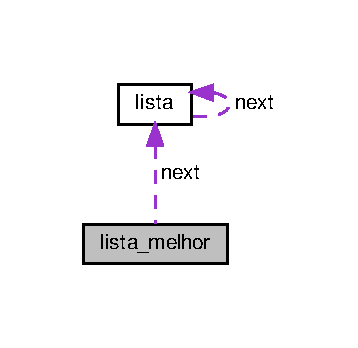
\includegraphics[width=172pt]{structlista__melhor__coll__graph}
\end{center}
\end{figure}
\subsection*{Public Attributes}
\begin{DoxyCompactItemize}
\item 
\mbox{\Hypertarget{structlista__melhor_a557aadd45cee0a0490d5b673711f05a0}\label{structlista__melhor_a557aadd45cee0a0490d5b673711f05a0}} 
void $\ast$ {\bfseries valor}
\item 
\mbox{\Hypertarget{structlista__melhor_a759e9837330b5d64135872541ba76a13}\label{structlista__melhor_a759e9837330b5d64135872541ba76a13}} 
void $\ast$ {\bfseries coord}
\item 
\mbox{\Hypertarget{structlista__melhor_a3660b043cab71e94bd50cbcf06231bde}\label{structlista__melhor_a3660b043cab71e94bd50cbcf06231bde}} 
struct \hyperlink{structlista}{lista} $\ast$ {\bfseries next}
\end{DoxyCompactItemize}


The documentation for this struct was generated from the following file\+:\begin{DoxyCompactItemize}
\item 
listas.\+h\end{DoxyCompactItemize}

\chapter{File Documentation}
\hypertarget{Interface_8h}{}\section{Interface.\+h File Reference}
\label{Interface_8h}\index{Interface.\+h@{Interface.\+h}}
{\ttfamily \#include \char`\"{}dados.\+h\char`\"{}}\newline
Include dependency graph for Interface.\+h\+:
\nopagebreak
\begin{figure}[H]
\begin{center}
\leavevmode
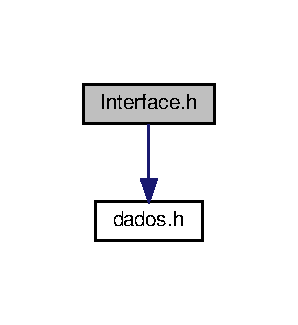
\includegraphics[width=143pt]{Interface_8h__incl}
\end{center}
\end{figure}
This graph shows which files directly or indirectly include this file\+:
\nopagebreak
\begin{figure}[H]
\begin{center}
\leavevmode
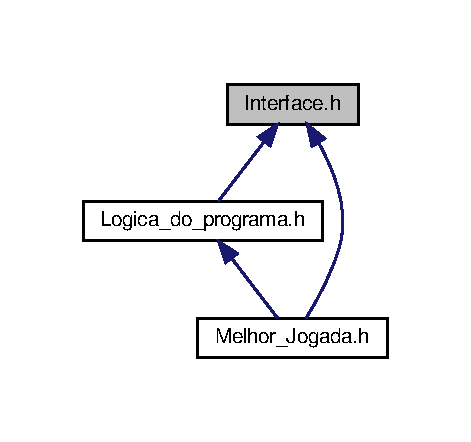
\includegraphics[width=226pt]{Interface_8h__dep__incl}
\end{center}
\end{figure}
\subsection*{Functions}
\begin{DoxyCompactItemize}
\item 
void \hyperlink{Interface_8h_a8d137184689f55d869b4fa543e76e70b}{mostra\+\_\+tabuleiro} (C\+A\+SA tab\mbox{[}8\mbox{]}\mbox{[}8\mbox{]}, F\+I\+LE $\ast$stream)
\begin{DoxyCompactList}\small\item\em T\+A\+B\+U\+L\+E\+I\+RO \+: I\+M\+P\+R\+I\+ME OU G\+U\+A\+R\+DA ///. \end{DoxyCompactList}\item 
void \hyperlink{Interface_8h_a7d93f27be42746f9ca9c2292b55e6aec}{jogador\+\_\+vencedor} (\hyperlink{structESTADO}{E\+S\+T\+A\+DO} $\ast$estado, F\+I\+LE $\ast$stream)
\begin{DoxyCompactList}\small\item\em J\+O\+G\+A\+D\+OR V\+E\+N\+C\+E\+D\+OR ///. \end{DoxyCompactList}\item 
\mbox{\Hypertarget{Interface_8h_a5da86839ee9a47cb34b275831d3cc1f9}\label{Interface_8h_a5da86839ee9a47cb34b275831d3cc1f9}} 
void \hyperlink{Interface_8h_a5da86839ee9a47cb34b275831d3cc1f9}{guarda\+\_\+tabuleiro} (\hyperlink{structESTADO}{E\+S\+T\+A\+DO} $\ast$estado, F\+I\+LE $\ast$stream)
\begin{DoxyCompactList}\small\item\em Guarda no ficheiro o tabuleiro do jogo, recorrendo à função guarda\+\_\+linha. \end{DoxyCompactList}\item 
\mbox{\Hypertarget{Interface_8h_acc259ba457da7c00c734bb9d079fad17}\label{Interface_8h_acc259ba457da7c00c734bb9d079fad17}} 
void \hyperlink{Interface_8h_acc259ba457da7c00c734bb9d079fad17}{prompt} (\hyperlink{structESTADO}{E\+S\+T\+A\+DO} $\ast$estado, F\+I\+LE $\ast$stream)
\begin{DoxyCompactList}\small\item\em Prompt do jogo. \end{DoxyCompactList}\item 
int \hyperlink{Interface_8h_a0475a591894db72239ed040e576d32b5}{interpretador} (\hyperlink{structESTADO}{E\+S\+T\+A\+DO} $\ast$estado)
\begin{DoxyCompactList}\small\item\em I\+N\+T\+E\+R\+P\+R\+E\+T\+A\+D\+OR ///. \end{DoxyCompactList}\end{DoxyCompactItemize}


\subsection{Detailed Description}
Definição do intrepretador do jogo. 

\subsection{Function Documentation}
\mbox{\Hypertarget{Interface_8h_a0475a591894db72239ed040e576d32b5}\label{Interface_8h_a0475a591894db72239ed040e576d32b5}} 
\index{Interface.\+h@{Interface.\+h}!interpretador@{interpretador}}
\index{interpretador@{interpretador}!Interface.\+h@{Interface.\+h}}
\subsubsection{\texorpdfstring{interpretador()}{interpretador()}}
{\footnotesize\ttfamily int interpretador (\begin{DoxyParamCaption}\item[{\hyperlink{structESTADO}{E\+S\+T\+A\+DO} $\ast$}]{estado }\end{DoxyParamCaption})}



I\+N\+T\+E\+R\+P\+R\+E\+T\+A\+D\+OR ///. 

Intrepretador do jogo. \mbox{\Hypertarget{Interface_8h_a7d93f27be42746f9ca9c2292b55e6aec}\label{Interface_8h_a7d93f27be42746f9ca9c2292b55e6aec}} 
\index{Interface.\+h@{Interface.\+h}!jogador\+\_\+vencedor@{jogador\+\_\+vencedor}}
\index{jogador\+\_\+vencedor@{jogador\+\_\+vencedor}!Interface.\+h@{Interface.\+h}}
\subsubsection{\texorpdfstring{jogador\+\_\+vencedor()}{jogador\_vencedor()}}
{\footnotesize\ttfamily void jogador\+\_\+vencedor (\begin{DoxyParamCaption}\item[{\hyperlink{structESTADO}{E\+S\+T\+A\+DO} $\ast$}]{estado,  }\item[{F\+I\+LE $\ast$}]{stream }\end{DoxyParamCaption})}



J\+O\+G\+A\+D\+OR V\+E\+N\+C\+E\+D\+OR ///. 

Função que determina o vencedor do jogo. \mbox{\Hypertarget{Interface_8h_a8d137184689f55d869b4fa543e76e70b}\label{Interface_8h_a8d137184689f55d869b4fa543e76e70b}} 
\index{Interface.\+h@{Interface.\+h}!mostra\+\_\+tabuleiro@{mostra\+\_\+tabuleiro}}
\index{mostra\+\_\+tabuleiro@{mostra\+\_\+tabuleiro}!Interface.\+h@{Interface.\+h}}
\subsubsection{\texorpdfstring{mostra\+\_\+tabuleiro()}{mostra\_tabuleiro()}}
{\footnotesize\ttfamily void mostra\+\_\+tabuleiro (\begin{DoxyParamCaption}\item[{C\+A\+SA}]{tab\mbox{[}8\mbox{]}\mbox{[}8\mbox{]},  }\item[{F\+I\+LE $\ast$}]{stream }\end{DoxyParamCaption})}



T\+A\+B\+U\+L\+E\+I\+RO \+: I\+M\+P\+R\+I\+ME OU G\+U\+A\+R\+DA ///. 

Função que que imprime apenas as pecas de um determinado tabuleiro . 
\hypertarget{Logica__do__programa_8h}{}\section{Logica\+\_\+do\+\_\+programa.\+h File Reference}
\label{Logica__do__programa_8h}\index{Logica\+\_\+do\+\_\+programa.\+h@{Logica\+\_\+do\+\_\+programa.\+h}}
{\ttfamily \#include \char`\"{}dados.\+h\char`\"{}}\newline
{\ttfamily \#include \char`\"{}Interface.\+h\char`\"{}}\newline
Include dependency graph for Logica\+\_\+do\+\_\+programa.\+h\+:
\nopagebreak
\begin{figure}[H]
\begin{center}
\leavevmode
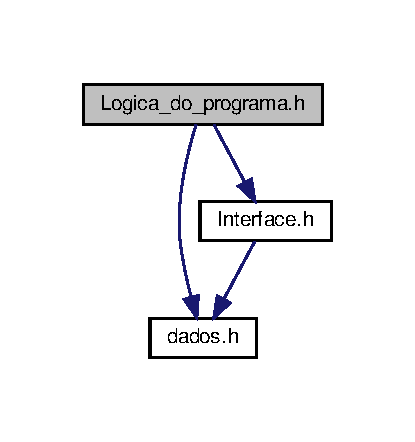
\includegraphics[width=199pt]{Logica__do__programa_8h__incl}
\end{center}
\end{figure}
This graph shows which files directly or indirectly include this file\+:
\nopagebreak
\begin{figure}[H]
\begin{center}
\leavevmode
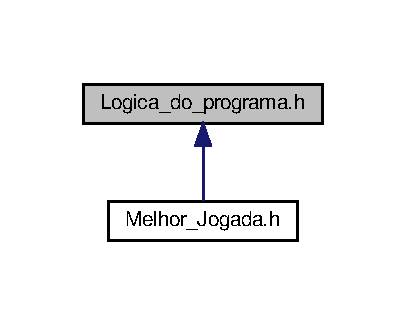
\includegraphics[width=195pt]{Logica__do__programa_8h__dep__incl}
\end{center}
\end{figure}
\subsection*{Functions}
\begin{DoxyCompactItemize}
\item 
void \hyperlink{Logica__do__programa_8h_acb9b7f916bd4759fb2de8b664f8bf447}{guarda\+\_\+\+Jogadas\+\_\+2} (\hyperlink{structESTADO}{E\+S\+T\+A\+DO} $\ast$estado, \hyperlink{structCOORDENADA}{C\+O\+O\+R\+D\+E\+N\+A\+DA} coord1, \hyperlink{structCOORDENADA}{C\+O\+O\+R\+D\+E\+N\+A\+DA} coord2, int n\+\_\+jogada)
\begin{DoxyCompactList}\small\item\em Função que guarda as jogadas do estado. \end{DoxyCompactList}\item 
\mbox{\Hypertarget{Logica__do__programa_8h_a922e98eb3acd7905b4adf8902d29283c}\label{Logica__do__programa_8h_a922e98eb3acd7905b4adf8902d29283c}} 
void \hyperlink{Logica__do__programa_8h_a922e98eb3acd7905b4adf8902d29283c}{guarda\+\_\+\+Jogadas\+\_\+1} (\hyperlink{structESTADO}{E\+S\+T\+A\+DO} $\ast$estado, \hyperlink{structCOORDENADA}{C\+O\+O\+R\+D\+E\+N\+A\+DA} coord1, int n\+\_\+jogada)
\begin{DoxyCompactList}\small\item\em Função que guarda as jogadas do estado. \end{DoxyCompactList}\item 
\mbox{\Hypertarget{Logica__do__programa_8h_a47b3e031aec8f1c2122a509d0248d655}\label{Logica__do__programa_8h_a47b3e031aec8f1c2122a509d0248d655}} 
void \hyperlink{Logica__do__programa_8h_a47b3e031aec8f1c2122a509d0248d655}{atualiza\+\_\+estado\+\_\+comando\+\_\+ler} (\hyperlink{structESTADO}{E\+S\+T\+A\+DO} $\ast$estado)
\begin{DoxyCompactList}\small\item\em Função que atualiza o estado lido através do comando ler. \end{DoxyCompactList}\item 
\mbox{\Hypertarget{Logica__do__programa_8h_ac9e0cf779056087992fbc75a05b93829}\label{Logica__do__programa_8h_ac9e0cf779056087992fbc75a05b93829}} 
void \hyperlink{Logica__do__programa_8h_ac9e0cf779056087992fbc75a05b93829}{mostra\+\_\+pos} (\hyperlink{structESTADO}{E\+S\+T\+A\+DO} $\ast$estado, int n\+\_\+jogadas)
\begin{DoxyCompactList}\small\item\em F\+U\+NÇÃO Q\+UE M\+O\+S\+T\+RA O P\+OS ///. \end{DoxyCompactList}\item 
\mbox{\Hypertarget{Logica__do__programa_8h_a793882e61a83db5efd6648dc25934546}\label{Logica__do__programa_8h_a793882e61a83db5efd6648dc25934546}} 
void \hyperlink{Logica__do__programa_8h_a793882e61a83db5efd6648dc25934546}{atualiza\+\_\+estado} (\hyperlink{structESTADO}{E\+S\+T\+A\+DO} $\ast$estado, \hyperlink{structCOORDENADA}{C\+O\+O\+R\+D\+E\+N\+A\+DA} coord\+\_\+mudar)
\begin{DoxyCompactList}\small\item\em Função que atualiza o estado a cada jogada. \end{DoxyCompactList}\item 
\mbox{\Hypertarget{Logica__do__programa_8h_aedac94896fa0c978db67ffa48463b731}\label{Logica__do__programa_8h_aedac94896fa0c978db67ffa48463b731}} 
int \hyperlink{Logica__do__programa_8h_aedac94896fa0c978db67ffa48463b731}{jogar} (\hyperlink{structESTADO}{E\+S\+T\+A\+DO} $\ast$estado, \hyperlink{structCOORDENADA}{C\+O\+O\+R\+D\+E\+N\+A\+DA} coord)
\begin{DoxyCompactList}\small\item\em Função que altera o estado do jogo cosoante a jogada efetuada. \end{DoxyCompactList}\item 
\mbox{\Hypertarget{Logica__do__programa_8h_a609da5e3c10cd0dccf9beb9533db2217}\label{Logica__do__programa_8h_a609da5e3c10cd0dccf9beb9533db2217}} 
void \hyperlink{Logica__do__programa_8h_a609da5e3c10cd0dccf9beb9533db2217}{atualiza\+\_\+estado\+\_\+pos} (\hyperlink{structESTADO}{E\+S\+T\+A\+DO} $\ast$estado, int n\+\_\+pos)
\begin{DoxyCompactList}\small\item\em Função que atualiza o estado em função do comando pos dado. \end{DoxyCompactList}\end{DoxyCompactItemize}


\subsection{Detailed Description}
Definição da função jogar responsável por alterar o estado do jogo. 

\subsection{Function Documentation}
\mbox{\Hypertarget{Logica__do__programa_8h_acb9b7f916bd4759fb2de8b664f8bf447}\label{Logica__do__programa_8h_acb9b7f916bd4759fb2de8b664f8bf447}} 
\index{Logica\+\_\+do\+\_\+programa.\+h@{Logica\+\_\+do\+\_\+programa.\+h}!guarda\+\_\+\+Jogadas\+\_\+2@{guarda\+\_\+\+Jogadas\+\_\+2}}
\index{guarda\+\_\+\+Jogadas\+\_\+2@{guarda\+\_\+\+Jogadas\+\_\+2}!Logica\+\_\+do\+\_\+programa.\+h@{Logica\+\_\+do\+\_\+programa.\+h}}
\subsubsection{\texorpdfstring{guarda\+\_\+\+Jogadas\+\_\+2()}{guarda\_Jogadas\_2()}}
{\footnotesize\ttfamily void guarda\+\_\+\+Jogadas\+\_\+2 (\begin{DoxyParamCaption}\item[{\hyperlink{structESTADO}{E\+S\+T\+A\+DO} $\ast$}]{estado,  }\item[{\hyperlink{structCOORDENADA}{C\+O\+O\+R\+D\+E\+N\+A\+DA}}]{coord1,  }\item[{\hyperlink{structCOORDENADA}{C\+O\+O\+R\+D\+E\+N\+A\+DA}}]{coord2,  }\item[{int}]{n\+\_\+jogada }\end{DoxyParamCaption})}



Função que guarda as jogadas do estado. 

C\+O\+M\+A\+N\+DO L\+ER /// A\+T\+U\+A\+L\+I\+ZA EM F\+U\+N\+C\+AO DO C\+O\+M\+A\+N\+DO L\+ER /// 
%--- End generated contents ---

% Index
\backmatter
\newpage
\phantomsection
\clearemptydoublepage
\addcontentsline{toc}{chapter}{Index}
\printindex

\end{document}
